\documentclass[tikz,border=10pt]{standalone}
\usetikzlibrary{calc}
\begin{document}
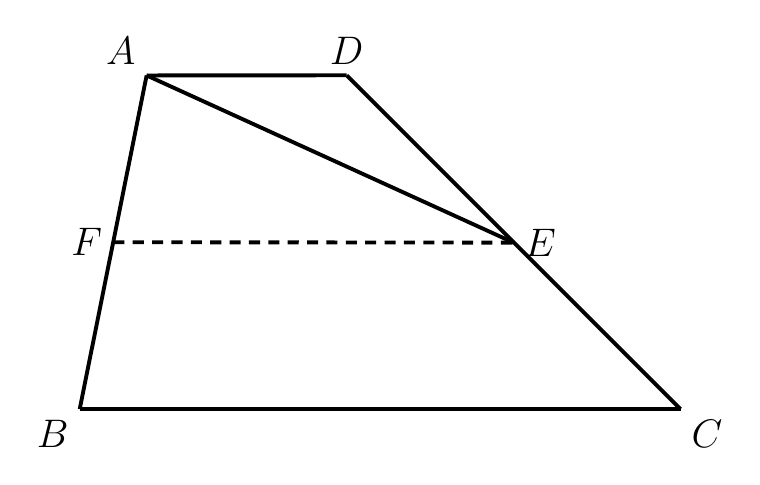
\begin{tikzpicture}[line width=1.4pt, line join=round]
  % Vertices (TikZ units, cm; s = 0.011976 per px, y flipped)
  \coordinate (A) at (-2.972,2.112);
  \coordinate (D) at (-0.431,2.114);
  \coordinate (B) at (-3.822,-2.126);
  \coordinate (C) at (3.808,-2.126);
  \coordinate (E) at (1.688,-0.011);
  \coordinate (F) at (-3.395,-0.006);

  % Solid edges
  \draw (A) -- (D);      % top
  \draw (D) -- (C);      % right side through E
  \draw (C) -- (B);      % bottom
  \draw (B) -- (A);      % left side
  \draw (A) -- (E);      % diagonal ending at E

  % Dashed horizontal at height of E: long dashes, clear gaps
  \draw[dash pattern=on 4pt off 3pt] (F) -- (E);

  % Labels
  \node[above left, font=\fontsize{14}{16.8}\selectfont] at (A) {$A$};
  \node[above, font=\fontsize{14}{16.8}\selectfont] at (D) {$D$};
  \node[below left, font=\fontsize{14}{16.8}\selectfont] at (B) {$B$};
  \node[below right, font=\fontsize{14}{16.8}\selectfont] at (C) {$C$};
  \node[left, font=\fontsize{14}{16.8}\selectfont] at (F) {$F$};
  % E label directly to the right of E, vertically centred on the dashed line
  \node[right, font=\fontsize{14}{16.8}\selectfont] at (E) {$E$};
\end{tikzpicture}
\end{document}